% Aplicar el estilo de página a todo el documento
\pagestyle{plain}
\section*{Introducción}
\addcontentsline{toc}{section}{Introducción}
Este manual tiene como objetivo proporcionar una guía clara y estructurada para la instalación, configuración y uso del Simulador de Laboratorio de Química Inorgánica en Realidad Virtual. Dirigido a estudiantes y profesores, detalla las funcionalidades y procedimientos necesarios para interactuar de manera eficiente con el sistema.

A través de este documento, el usuario podrá comprender las características principales del simulador, las herramientas disponibles y los pasos para realizar experimentos químicos en un entorno virtual controlado. Además, se incluyen recomendaciones prácticas y soluciones a posibles problemas para optimizar su experiencia.

\section{Requisitos del Sistema}
Para garantizar una experiencia óptima, el simulador requiere las siguientes especificaciones en dispositivos de realidad virtual compatibles:

\subsection{Especificaciones Técnicas}
\begin{itemize}
    \item \textbf{Dispositivos Compatibles}:
    \begin{itemize}
        \item Meta Quest 2
        \item Meta Quest Pro
        \item Meta Quest 3
    \end{itemize}
    \item \textbf{Espacio de Almacenamiento}: 450 MB disponibles en el dispositivo.
    \item \textbf{Zona de Uso Requerida}: Área libre de obstáculos con un mínimo de 2x2 metros.
\end{itemize}

\subsection{Recomendaciones}
Utilizar en un entorno con iluminación adecuada para un mejor rendimiento del sistema de seguimiento de manos (hand tracking).
\newpage
\section{Configuración e Instalación}

Esta sección detalla los pasos necesarios para instalar el simulador en dispositivos de realidad virtual compatibles y preparar el entorno para su correcto funcionamiento.

\subsection{Instalación de la Aplicación}

Para instalar la aplicación del simulador, utilizaremos SideQuest, una plataforma que permite cargar aplicaciones externas en las gafas de realidad virtual. A continuación, se describen los pasos para realizar la instalación:

\begin{enumerate}
    \item \textbf{Descarga e Instalación de SideQuest:}
    \begin{itemize}
        \item Acceda al sitio web oficial de SideQuest: \url{https://sidequestvr.com/setup-howto}.
        \item Descargue la versión adecuada de SideQuest para su sistema operativo.
        \item Instale SideQuest siguiendo las instrucciones proporcionadas en el sitio web.
    \end{itemize}
    \begin{figure}[thbp]
        \centering
        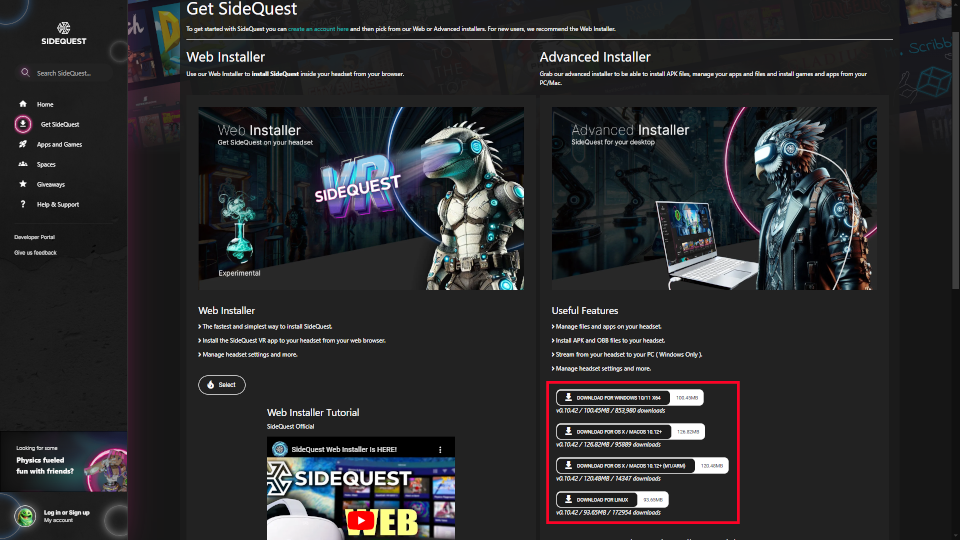
\includegraphics[width=0.75\textwidth, height = 7cm]{img/Configuración/Side_Quest (2).png}
        \caption{Web Oficial de SideQuest}
        \label{fig:Web Oficial de SideQuest}
    \end{figure}
    \newpage
    \item \textbf{Configuración del Modo Desarrollador en las Gafas}

    Para habilitar el modo desarrollador, es necesario utilizar la aplicación móvil \textit{Meta Horizon}. Siga los pasos a continuación para realizar esta configuración:
    
    \begin{enumerate}[I]
        \item Descargue la aplicación \textit{Meta Horizon} desde la \textbf{Play Store} (dispositivos Android) o la \textbf{App Store} (dispositivos iOS).  
        \item Abra la aplicación, ingrese con una cuenta de Meta y acceda al menú principal.  
        \item Seleccione la opción \textbf{Dispositivos}.  
        \begin{figure}[thbp]
            \centering
            \begin{subfigure}[b]{0.3\linewidth}
                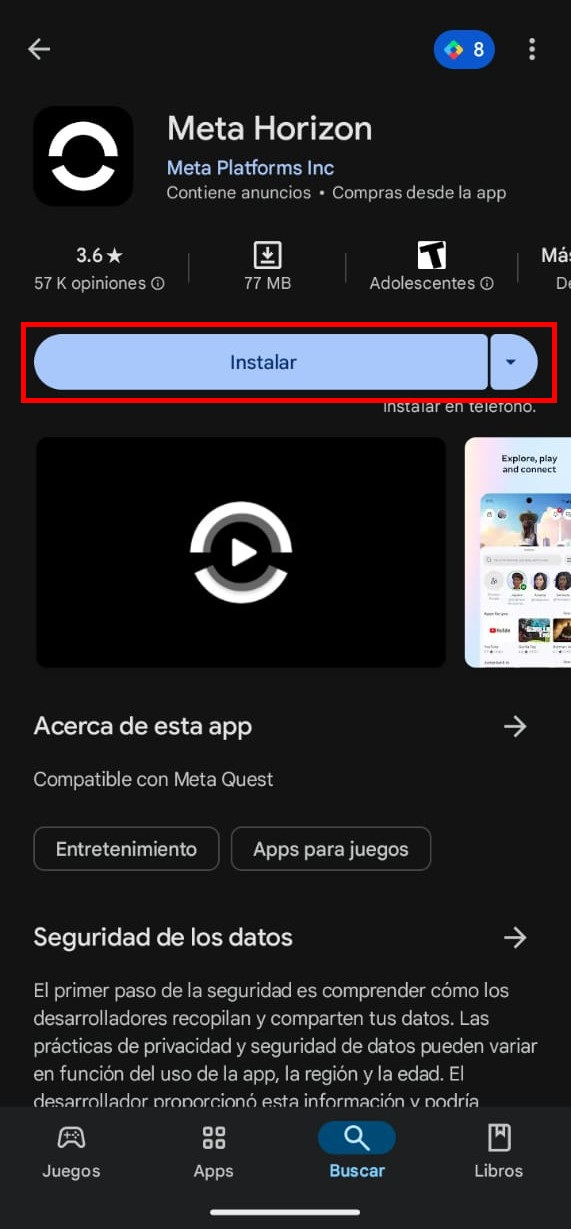
\includegraphics[width=\linewidth, height = 8cm]{img/Configuración/Instalacion_Meta.jpg}
            \end{subfigure}
            \begin{subfigure}[b]{0.3\linewidth}
                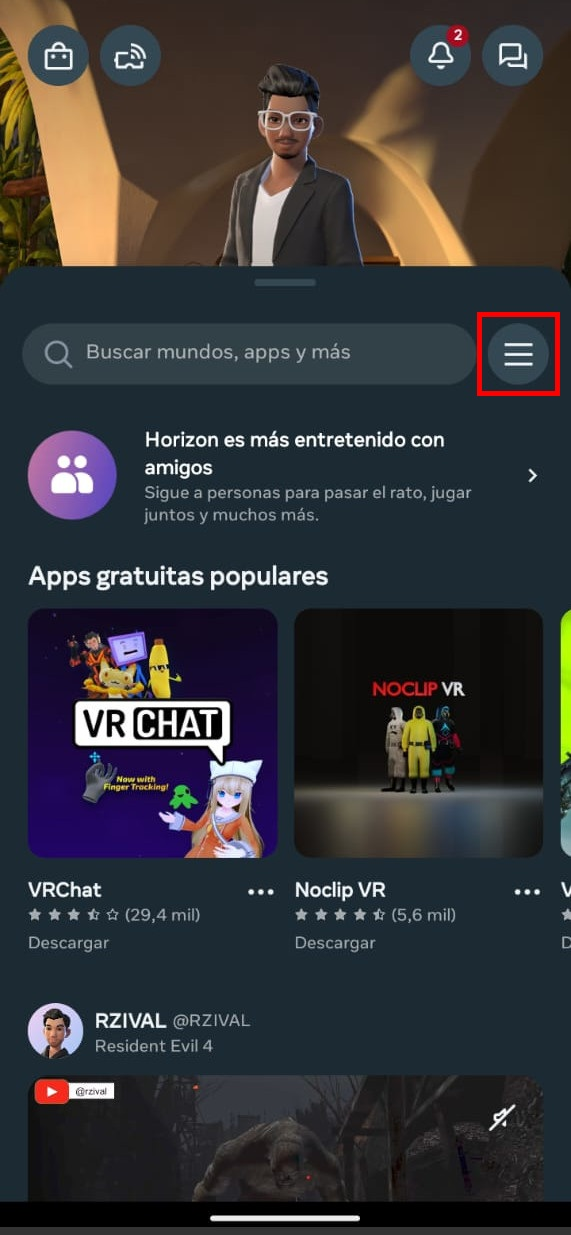
\includegraphics[width=\linewidth, height = 8cm]{img/Configuración/Hub_Meta.jpg}
            \end{subfigure}
            \begin{subfigure}[b]{0.3\linewidth}
                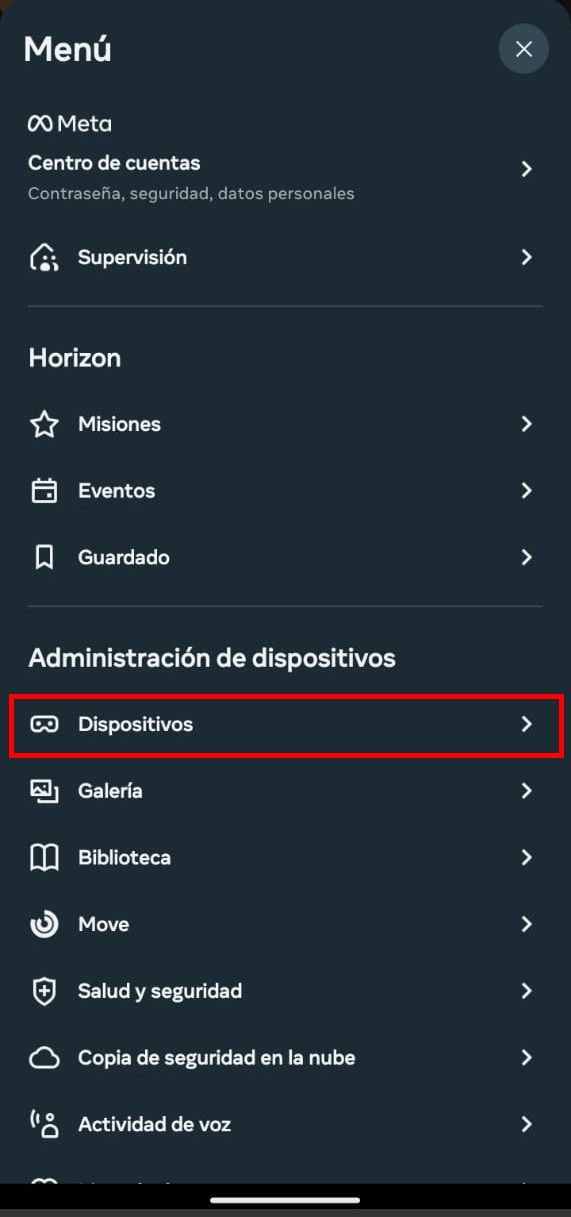
\includegraphics[width=\linewidth, height = 8cm]{img/Configuración/Menu_Meta.jpg}
            \end{subfigure}
            \caption{Configuración del Modo Desarrollador}
        \end{figure}
        \item Elija \textbf{Agregar dispositivo} y siga las instrucciones en pantalla para emparejar sus gafas con la aplicación.  
        \item Seleccione el modelo de sus gafas (Meta Quest 2, Meta Quest Pro o Meta Quest 3) de la lista de dispositivos disponibles.  
        \begin{figure}[thbp]
            \centering
            \begin{subfigure}[b]{0.3\linewidth}
                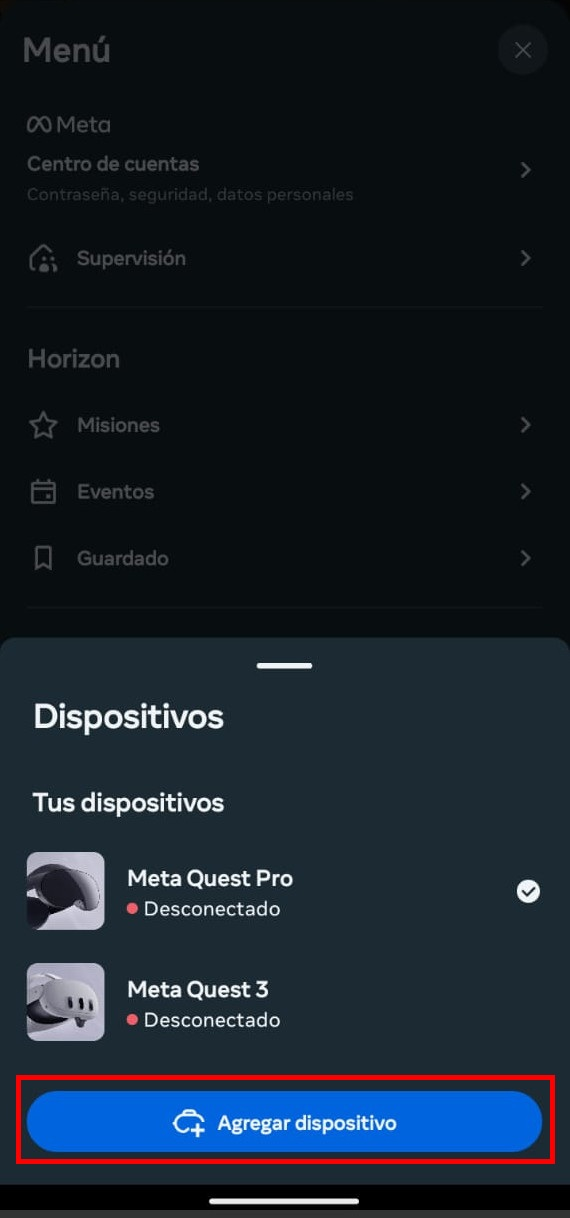
\includegraphics[width=\linewidth, height = 7cm]{img/Configuración/Dispositivos_Meta.jpg}
            \end{subfigure}
            \begin{subfigure}[b]{0.3\linewidth}
                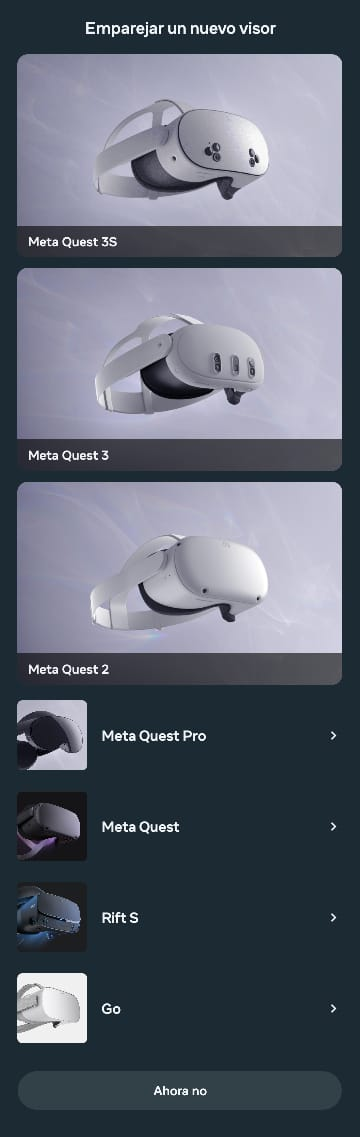
\includegraphics[width=\linewidth, height = 7cm]{img/Configuración/Emparejar_Dispositivos.jpg}
            \end{subfigure}
            \caption{Emparejamiento de Dispositivo}
        \end{figure}
        \item Una vez emparejadas las gafas, acceda a las opciones de configuración y active el \textbf{Modo Desarrollador}.  
        \begin{figure}[thbp]
            \centering
            \begin{subfigure}[b]{0.3\linewidth}
                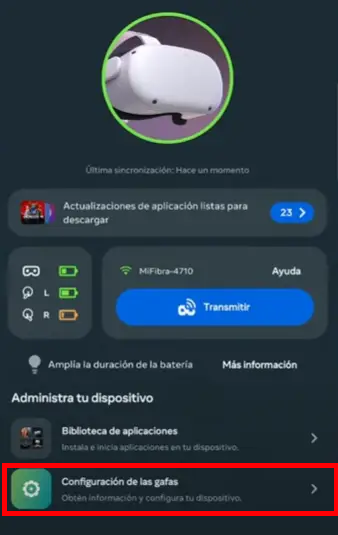
\includegraphics[width=\linewidth, height = 8cm]{img/Configuración/Modo_desarrollador.png}
            \end{subfigure}
            \begin{subfigure}[b]{0.3\linewidth}
                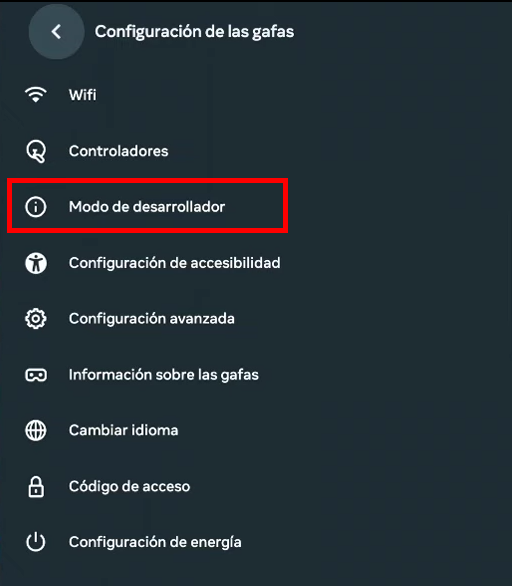
\includegraphics[width=\linewidth, height = 8cm]{img/Configuración/Modo_Desarrollador (2).png}
            \end{subfigure}
            \caption{Activacion del modo desarrollador}
        \end{figure}
    \end{enumerate}

    \item \textbf{Conexión de las Gafas al Ordenador:}
    \begin{itemize}
        \item Conecte las gafas de realidad virtual al ordenador mediante un cable USB.
        \item En las gafas, aparecerá una solicitud para permitir la depuración USB; seleccione \textit{Permitir}.
    \end{itemize}
    \item \textbf{Instalación de la Aplicación desde el Ordenador:}
    \begin{itemize}
        \item Abra SideQuest en su ordenador.
        \item Asegúrese de que SideQuest reconozca las gafas; un indicador verde en la esquina superior izquierda confirmará la conexión exitosa.
        \item Haga clic en el ícono de \textit{Instalar APK desde el ordenador} (ícono de una flecha hacia abajo).
        \begin{figure}[thbp]
            \centering
            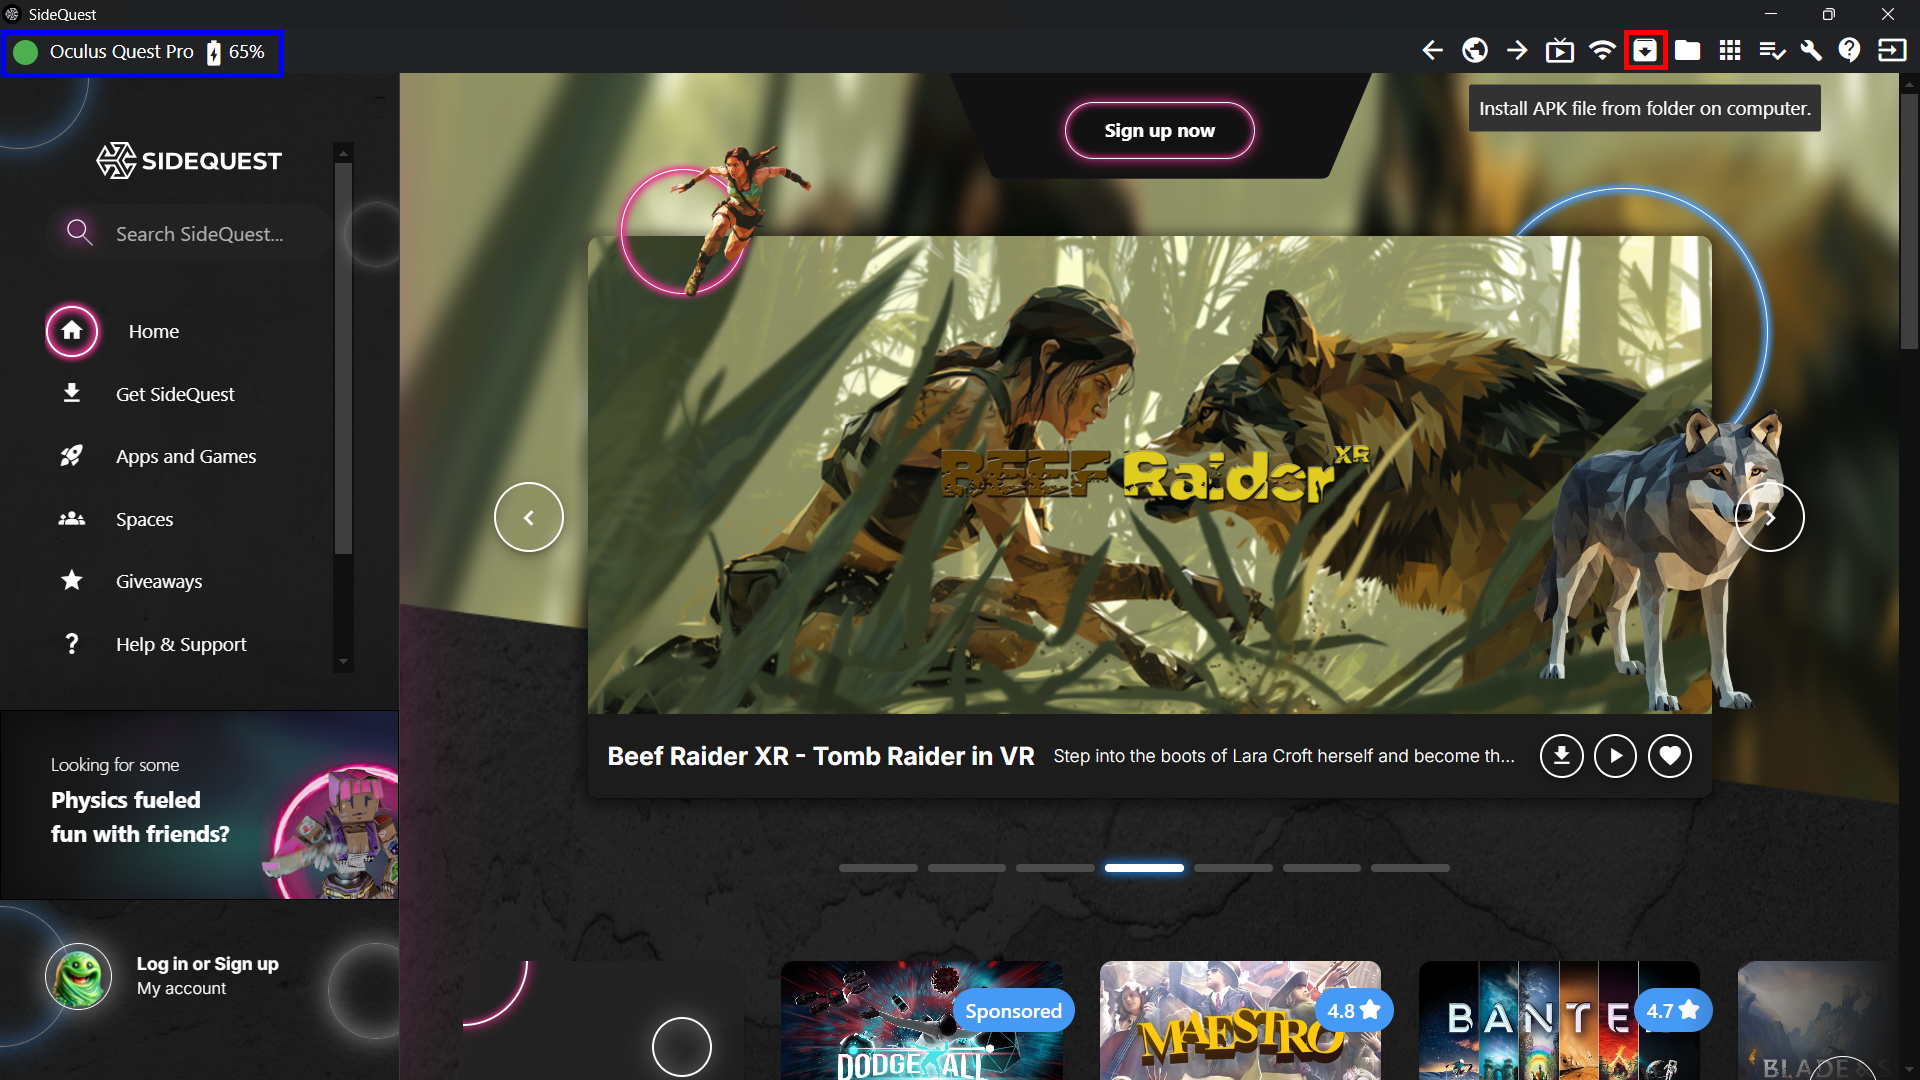
\includegraphics[width=0.75\textwidth, height = 6cm]{img/Configuración/Hub_SideQuest.png}
            \caption{Instalación del Apk}
            \label{fig:Instalación del Apk}
        \end{figure}
        \item Seleccione el archivo APK del simulador almacenado en su ordenador.
        \item Espere a que la instalación se complete; SideQuest notificará cuando el proceso haya finalizado.
        \begin{figure}[thbp]
            \centering
            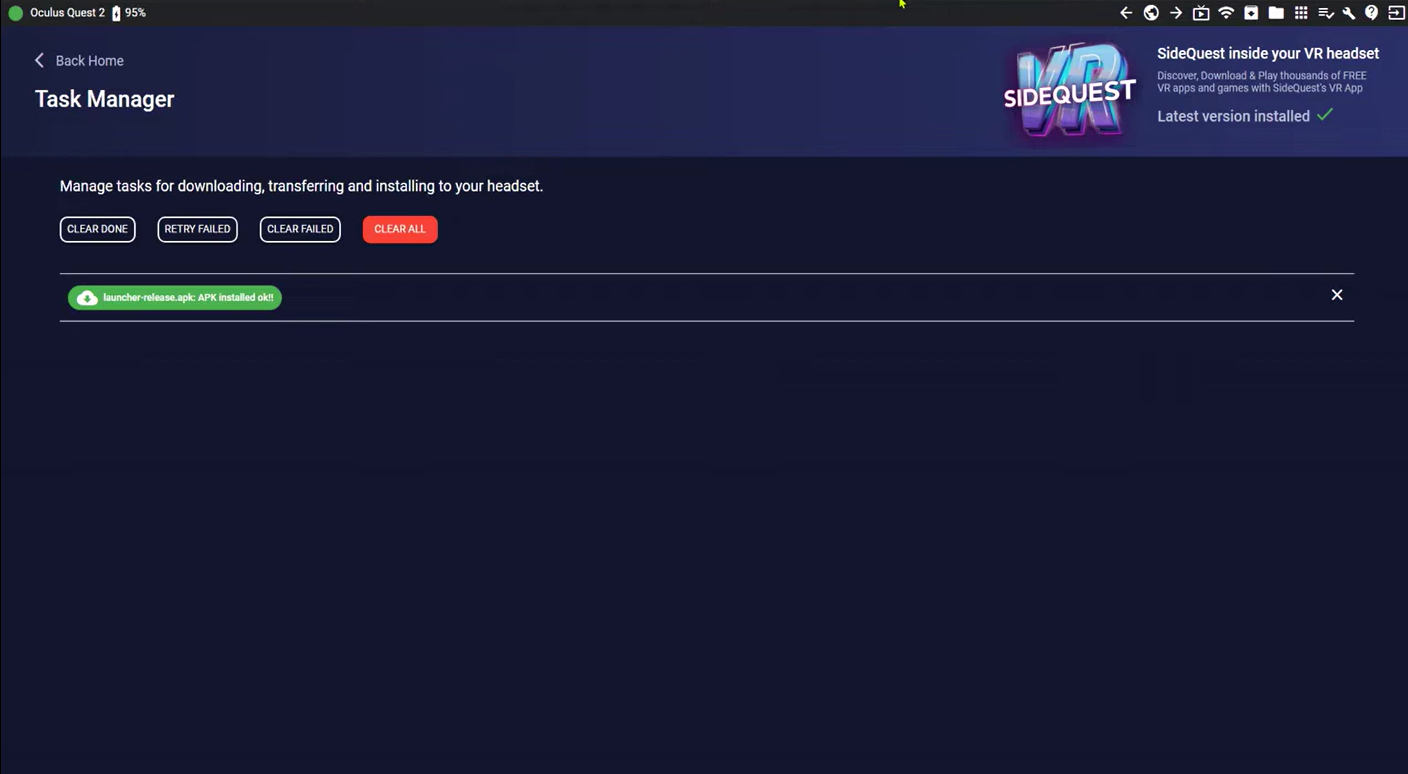
\includegraphics[width=0.75\textwidth, height = 6cm]{img/Configuración/Install_Complete.png}
            \caption{Instalación Completa}
            \label{fig:Instalación Completa}
        \end{figure}
    \end{itemize}
    \item \textbf{Verificación de la Instalación:}
    \begin{itemize}
        \item Desconecte las gafas del ordenador.
        \item Póngase las gafas y navegue hasta la sección de \textit{Aplicaciones}.
        \item En el menú desplegable de fuentes, seleccione \textit{Origen desconocido}.
        \item Localice y ejecute la aplicación del simulador desde la lista.
    \end{itemize}
    \begin{figure}[thbp]
            \centering
            \begin{subfigure}[b]{0.45\linewidth}
                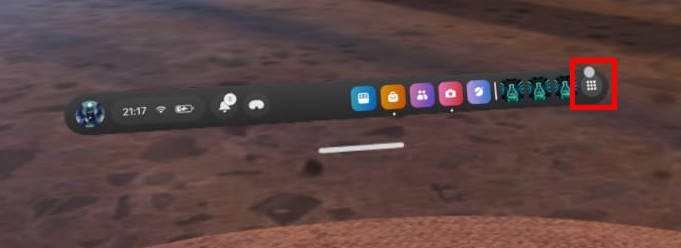
\includegraphics[width=\linewidth, height = 4cm]{img/Configuración/hub_oculus.jpg}
            \end{subfigure}
            \begin{subfigure}[b]{0.45\linewidth}
                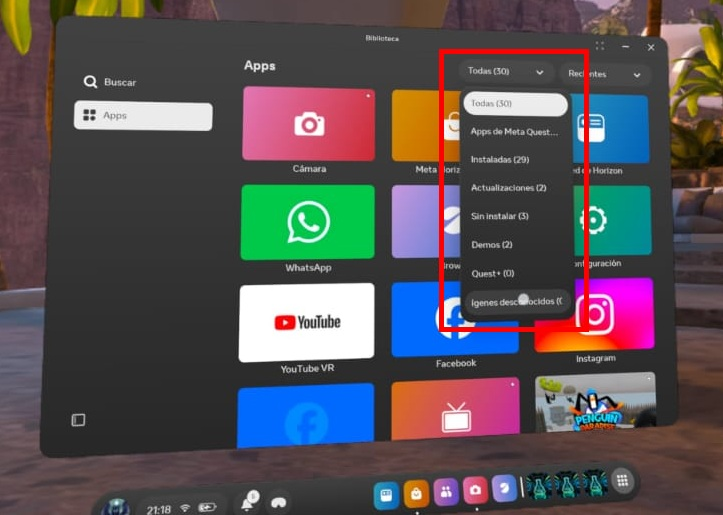
\includegraphics[width=\linewidth, height = 4cm]{img/Configuración/apps.jpg}
            \end{subfigure}
            \begin{subfigure}[b]{0.6\linewidth}
                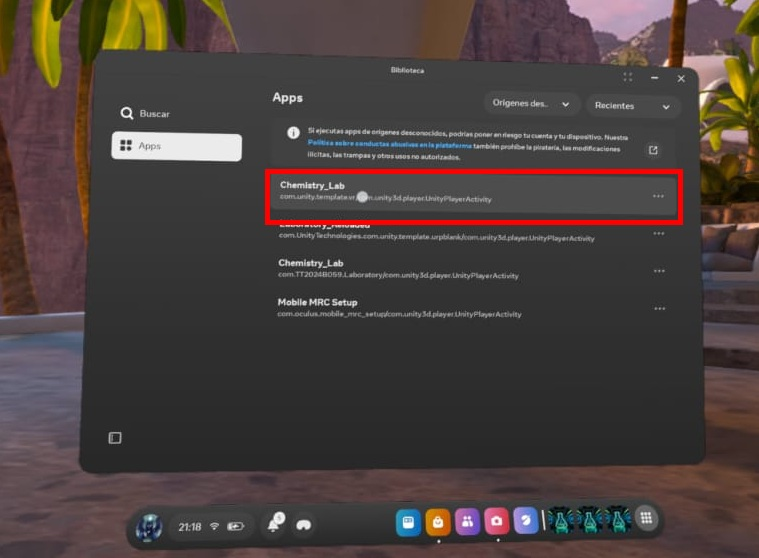
\includegraphics[width=\linewidth, height = 5cm]{img/Configuración/origenes_desconocidos.jpg}
            \end{subfigure}
            \caption{Verificación de la Instalación}
        \end{figure}
\end{enumerate}

\subsection{Configuración Inicial}

Antes de utilizar el simulador, es necesario preparar las gafas y el entorno de uso:

\begin{enumerate}
    \item \textbf{Calibración del Visor:}
    \begin{itemize}
        \item Ajuste las correas del visor para un ajuste cómodo y seguro.
        \item Realice la configuración inicial del visor si no se ha realizado previamente.
    \end{itemize}
    \item \textbf{Definición de la Zona de Uso:}
    \begin{itemize}
        \item Active el sistema \textit{Guardian} en las gafas.
        \item Seleccione la opción de \textbf{límite fijo}, especialmente recomendada para el uso del simulador, ya que permite definir un espacio estático y reduce distracciones durante las sesiones.
        \item Asegúrese de que el área delimitada esté libre de obstáculos como muebles, cables u objetos que puedan interferir con su experiencia.
    \end{itemize}
    \item \textbf{Configuración del Seguimiento de Manos:}
    \begin{itemize}
        \item Active el seguimiento de manos desde el menú de configuración del visor.
        \item Realice pruebas rápidas para garantizar que el sistema reconozca correctamente los gestos de sus manos.
    \end{itemize}
\end{enumerate}
\newpage
\section{Interfaces}

El simulador de laboratorio de química inorgánica en realidad virtual cuenta con diversas interfaces diseñadas para guiar al usuario durante la navegación y ejecución de los experimentos. A continuación, se describen las principales pantallas y sus funciones:

\subsection{Menú Principal}
El menú principal es la pantalla inicial del simulador, desde donde el usuario puede acceder a las funciones principales. Esta interfaz ofrece las siguientes opciones:
\begin{itemize}
    \item \textbf{Tutorial:} Dirige al usuario a una guía introductoria que explica cómo utilizar el simulador.
    \item \textbf{Lista de Experimentos:} Presenta las actividades disponibles para su selección.
\end{itemize}
\begin{figure}[thbp]
    \centering
    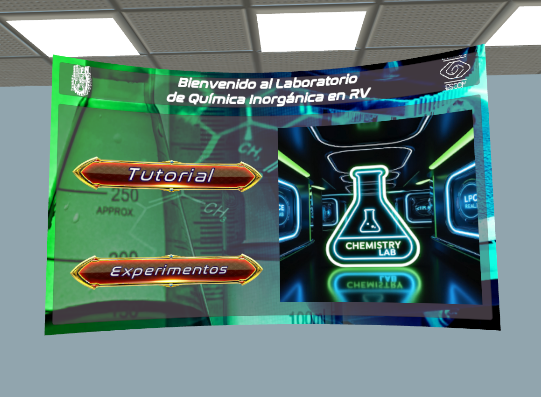
\includegraphics[width=0.5\textwidth, height = 5cm]{img/GUI/UI_Hub.png}
    \caption{Menú Principal}
    \label{fig:Menú_Principal}
\end{figure}

\subsection{Lista de Experimentos}
La lista de experimentos permite al usuario visualizar y seleccionar las actividades experimentales disponibles.
\textbf{Elementos principales:}
\begin{itemize}
    \item \textbf{Lista de Opciones:} Cada experimento aparece como un botón con su título correspondiente.
    \item \textbf{Botón de Regreso:} Ubicado en la parte inferior, permite regresar al Menú Principal.
\end{itemize}
\begin{figure}[thbp]
    \centering
    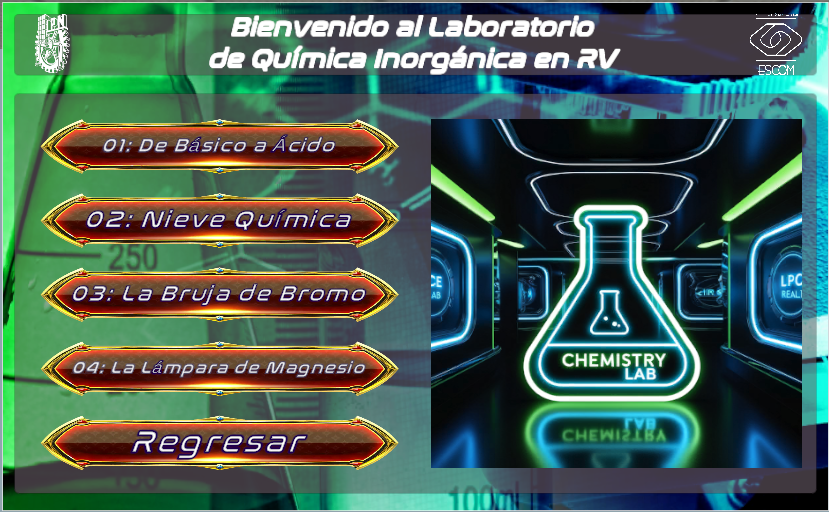
\includegraphics[width=0.5\textwidth, height = 5cm]{img/GUI/UI_Hub_Experiments (2).png}
    \caption{Menú Selección De Experimentos}
    \label{fig:Selección_De_Experimentos}
\end{figure}
Al seleccionar un experimento, el usuario será redirigido a la \textbf{pantalla de información} del experimento elegido.
\newpage

\subsection{Pantalla de Información}
Esta pantalla aparece después de seleccionar un tutorial o experimento. Su propósito es proporcionar una breve introducción antes de comenzar la actividad.
\textbf{Elementos principales:}
\begin{itemize}
    \item \textbf{Título:} Nombre del tutorial o experimento.
    \item \textbf{Descripción:} Breve introducción que explica el objetivo de la actividad seleccionada.
    \item \textbf{Opciones de Navegación:}
    \begin{itemize}
        \item \textbf{Regresar al Menú Principal:} Permite volver al menú inicial.
        \item \textbf{Confirmar Selección:} Inicia la actividad seleccionada.
    \end{itemize}
\end{itemize}
\begin{figure}[thbp]
    \centering
    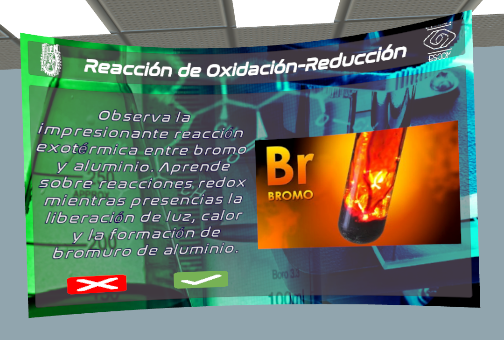
\includegraphics[width=0.5\textwidth, height = 5cm]{img/GUI/UI_Hub_Experiment.png}
    \caption{Información Del Experimento}
    \label{fig:Información_Del_Experimento}
\end{figure}
\newpage
\subsection{Pantalla Principal de Experimentos}
Durante la ejecución de un experimento, esta interfaz presenta las instrucciones y la ecuación química que el usuario debe balancear.
\textbf{Elementos principales:}
\begin{itemize}
    \item \textbf{Instrucciones:} Pasos detallados para realizar el experimento.
    \item \textbf{Ecuación Química a Balancear:} Mostrada en la parte superior de la pantalla, con campos interactuables para ingresar los coeficientes necesarios.
\end{itemize}
\begin{figure}[thbp]
    \centering
    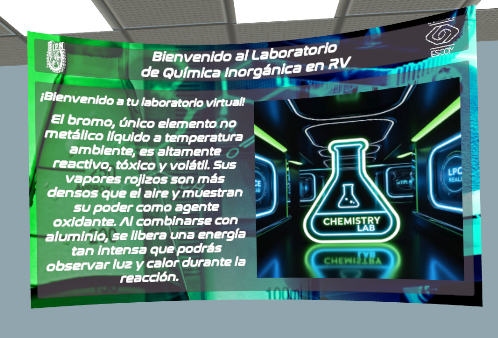
\includegraphics[width=0.5\textwidth, height = 5cm]{img/GUI/UI_Principal.png}
    \caption{Pantalla De Instrucciones}
    \label{fig:Pantalla_De_Instrucciones}
\end{figure}

\subsection{Teclado Numérico Interactivo (Numpad)}
Esta interfaz permite ingresar valores numéricos para el balanceo de ecuaciones químicas.
\begin{itemize}
    \item \textbf{Botones Numéricos:} Teclas del 0 al 9 para ingresar coeficientes.
    \item \textbf{Botón Validar:} Confirma el valor ingresado.
    \item \textbf{Botón Borrar:} Elimina el valor actual.
\end{itemize}
\begin{figure}[thbp]
    \centering
    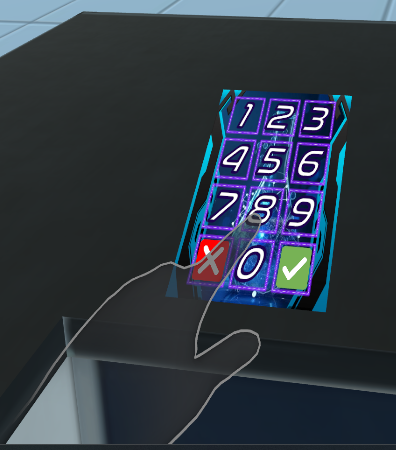
\includegraphics[width=0.5\textwidth, height = 5cm]{img/GUI/Num_Pad.png}
    \caption{Teclado Numérico}
    \label{fig:Teclado_Numérico}
\end{figure}
\newpage
\subsection{Información del Último Elemento Seleccionado}
Al seleccionar un elemento químico, esta interfaz presenta información relevante sobre el mismo.
\textbf{Elementos principales:}
\begin{itemize}
    \item \textbf{Nombre y Símbolo:} Identificación básica del elemento.
    \item \textbf{Propiedades Principales:} Información clave como número atómico, masa y clasificación.
    \item \textbf{Imagen de Referencia:} Representación visual del elemento seleccionado.
\end{itemize}
\begin{figure}[thbp]
    \centering
    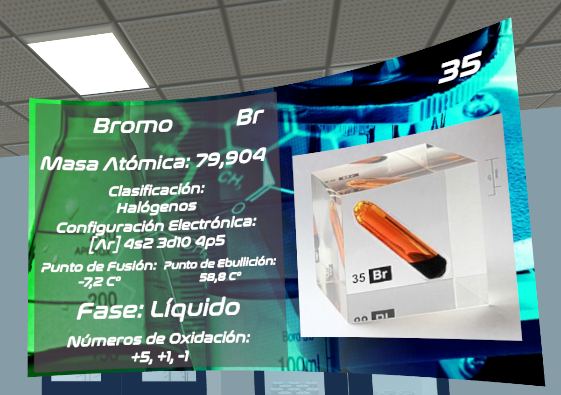
\includegraphics[width=0.5\textwidth, height = 5cm]{img/GUI/UI_Elements.png}
    \caption{Información Elementos}
    \label{fig:Información_Elementos}
\end{figure}
\subsection{Tabla Periódica 3D Interactiva}
La tabla periódica interactiva es una herramienta clave para la selección de elementos químicos.
\textbf{Funciones principales:}
\begin{itemize}
    \item \textbf{Selección de Elementos:} Los usuarios pueden seleccionar un elemento químico tocando directamente su ficha en el modelo tridimensional.
    \item \textbf{Visualización de Propiedades:} La información del elemento seleccionado se muestra automáticamente en la interfaz de "Información del Último Elemento Seleccionado".
\end{itemize}
\begin{figure}[thbp]
    \centering
    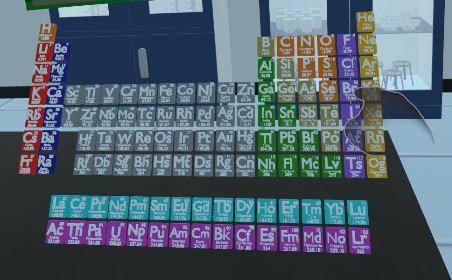
\includegraphics[width=0.5\textwidth, height = 5cm]{img/GUI/Tabla_Periodica.png}
    \caption{Tabla Periódica}
    \label{fig:Tabla_Periódica}
\end{figure}
\subsection{Información del Último Compuesto Creado}
Cuando se genera un compuesto válido, esta pantalla muestra detalles importantes del mismo.
\textbf{Elementos principales:}
\begin{itemize}
    \item \textbf{Nombre del Compuesto:} Identificación química del compuesto generado.
    \item \textbf{Propiedades Químicas:} Datos clave sobre su composición.
    \item \textbf{Imagen de Referencia:} Representación visual del compuesto.
\end{itemize}
\begin{figure}[thbp]
    \centering
    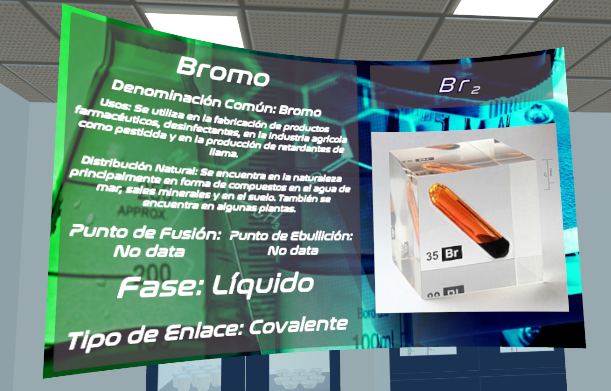
\includegraphics[width=0.5\textwidth, height = 5cm]{img/GUI/UI_Compuestos.png}
    \caption{Información Compuestos}
    \label{fig:Información_Compuestos}
\end{figure}
\subsection{Zona de Creación de Compuestos}
Esta interfaz permite combinar elementos químicos para formar compuestos válidos según los requisitos del experimento.
\begin{itemize}
    \item \textbf{Lista de Elementos Actuales:} Muestra los elementos que se han añadido a la zona de creación..
    \item \textbf{Botón de Creación:} Permite generar un compuesto químico cuando la combinación es válida.
    \item \textbf{Indicadores de Validez:} Si la combinación de elementos es válida, el botón de creación estará activo; en caso contrario, permanecerá inactivo.
\end{itemize}
\begin{figure}[thbp]
    \centering
    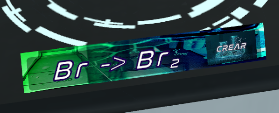
\includegraphics[width=0.5\textwidth, height = 5cm]{img/GUI/UI_Creacion.png}
    \caption{Creación de Compuestos}
    \label{fig:Creación_de_Compuestos}
\end{figure}
\subsection{Pantalla de Finalización del Experimento}
Al completar un experimento, esta pantalla ofrece las siguientes opciones:
\begin{itemize}
    \item \textbf{Repetir Experimento:} Permite reiniciar la actividad actual.
    \item \textbf{Regresar al Menú Principal:} Finaliza la actividad y redirige al menú inicial.
\end{itemize}
\begin{figure}[thbp]
    \centering
    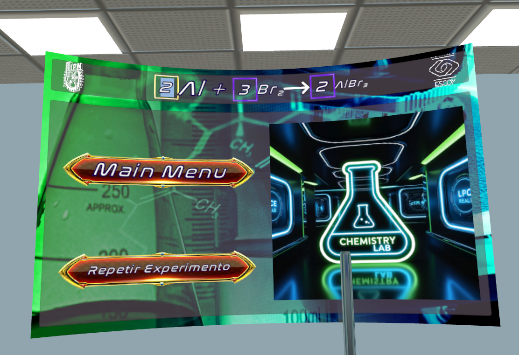
\includegraphics[width=0.5\textwidth, height = 5cm]{img/GUI/UI_Final.png}
    \caption{Menú Final Del Experimento}
    \label{fig:Menú_Final_Del_Experimento}
\end{figure}
\section{Interacción y Uso del Simulador}

El simulador de laboratorio de química inorgánica en realidad virtual está diseñado para ser intuitivo y altamente interactivo. A continuación, se describen los gestos, las principales interacciones y las funcionalidades disponibles en el simulador.

\subsection{Gestos Disponibles}

El simulador utiliza un sistema de seguimiento de manos que permite interactuar de manera natural con el entorno virtual. A continuación, se describen los gestos principales y su función:

\begin{itemize}
    \item \textbf{Centrado de Vista y Menú de Meta:}  
    Con la mano derecha, une el dedo índice y el pulgar formando un círculo, manteniendo los demás dedos extendidos y la palma hacia ti.  
    \begin{itemize}
        \item \textit{Centrado de Vista:} Mantén el gesto durante unos segundos para alinear el centro de la vista con el origen del sistema.  
        \item \textit{Menú de Meta:} Realiza el gesto una sola vez para abrir el menú principal del visor, donde puedes acceder a configuraciones y aplicaciones.  
    \end{itemize}
    \begin{figure}[thbp]
        \centering
        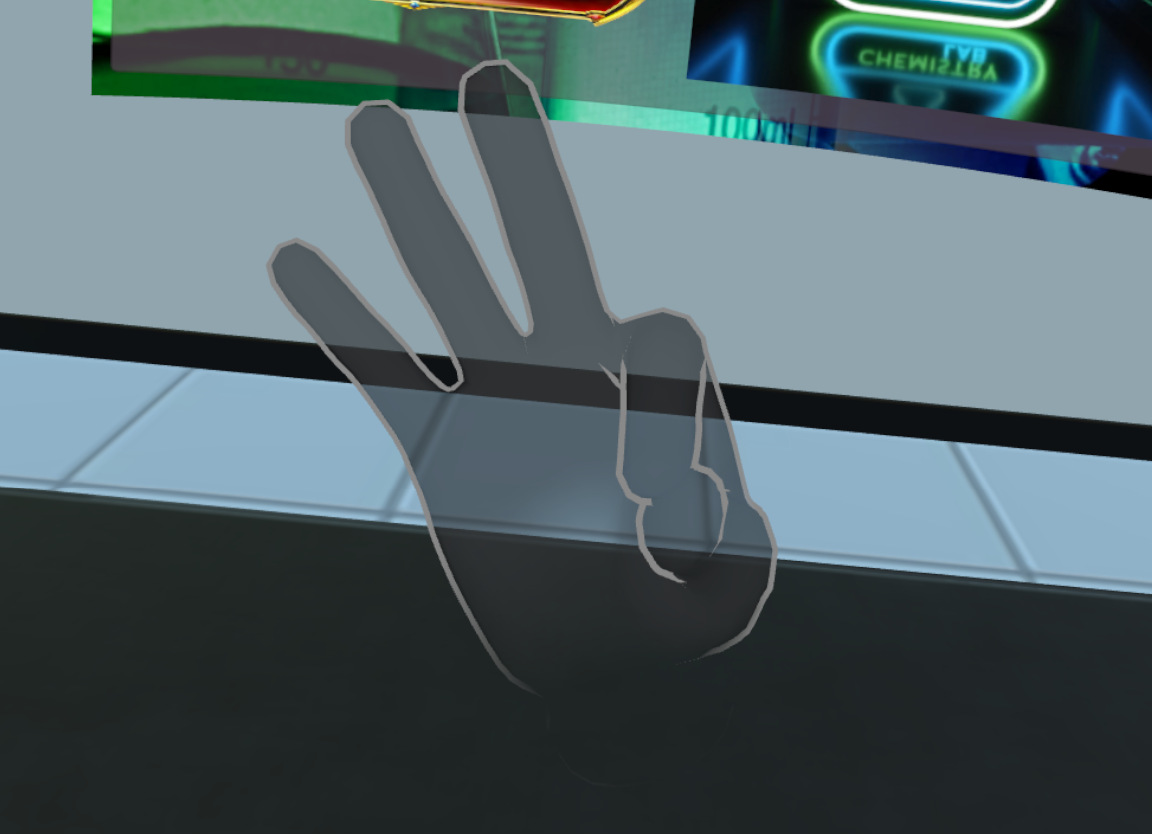
\includegraphics[width=0.45\textwidth, height = 3cm]{img/Interacciones/Centrado.png}
        \caption{Gesto Meta}
        \label{fig:Gesto Meta}
    \end{figure}
    \item \textbf{Agarre:}  
    Este gesto permite manipular objetos en el entorno virtual y puede realizarse de dos maneras:  
    \begin{itemize}
        \item \textit{Agarre Completo:} Cierra completamente la mano alrededor del objeto. Es ideal para recipientes y herramientas grandes.  
        \item \textit{Agarre de Pinza:} Une el dedo índice y el pulgar alrededor del objeto. Es más adecuado para elementos pequeños o delicados.  
    \end{itemize}
    \begin{figure}[thbp]
        \centering
        \begin{subfigure}[b]{0.4\linewidth}
            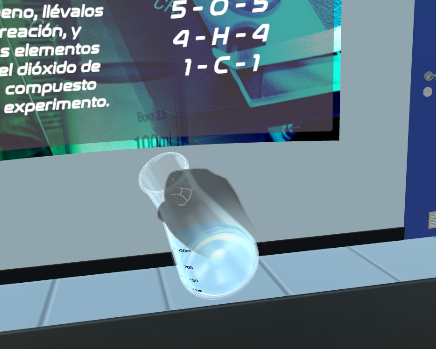
\includegraphics[width=\linewidth, height = 5cm]{img/Interacciones/Sujeción_Completa.png}
            \caption{Sujeción Completa}
            \label{fig:Sujeción_Completa}
        \end{subfigure}
        \begin{subfigure}[b]{0.4\linewidth}
            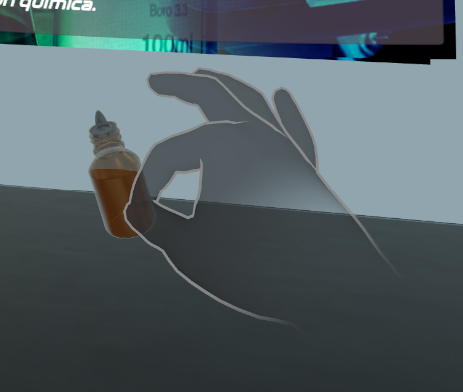
\includegraphics[width=\linewidth, height = 5cm]{img/Interacciones/Pinch (2).png}
            \caption{Sujeción de Pinza}
            \label{fig:Sujeción_Pinza}
        \end{subfigure}
        \caption{Tipos de Agarre}
    \end{figure}
    Para liberar un objeto, abre completamente la mano independientemente del tipo de agarre utilizado.

    \item \textbf{Interacción Lejana:}  
    Une el dedo índice y el pulgar de la mano derecha para interactuar con botones o campos fuera del alcance directo. Apunta con el cursor hacia el elemento deseado y realiza el gesto para confirmar la acción.
    \begin{figure}[thbp]
        \centering
        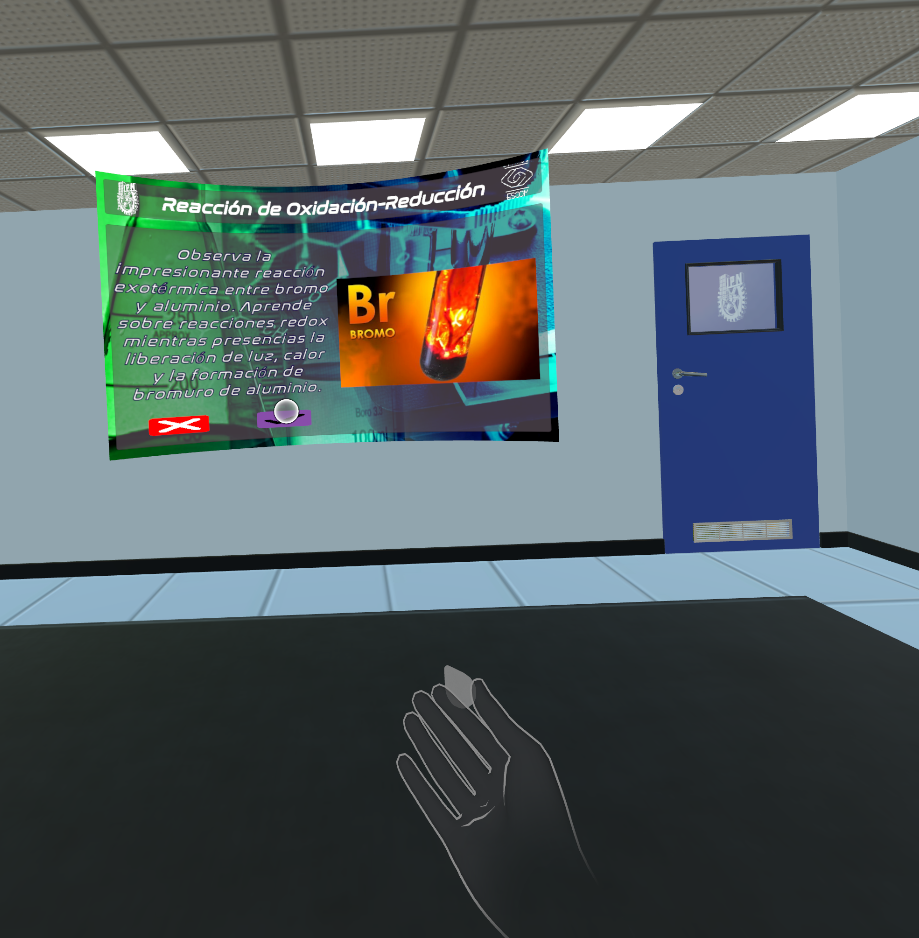
\includegraphics[width=0.5\textwidth, height = 5cm]{img/Interacciones/Apuntado_Manos.png}
        \caption{Apuntado}
        \label{fig:Apuntado}
    \end{figure}
    \item \textbf{Toque Directo:}  
    Utiliza el dedo índice para tocar directamente botones o interfaces cercanas. Este gesto también se usa para seleccionar elementos en la tabla periódica interactiva.
\end{itemize}
\newpage
\subsection{Acciones e Interacciones}

El simulador incluye diversas acciones diseñadas para replicar procedimientos comunes de laboratorio. A continuación, se describen las principales interacciones:

\begin{itemize}
    \item \textbf{Validar el Balanceo de Ecuaciones:}  
    Cuando estés seguro de los coeficientes ingresados, presiona el botón \textbf{Validar}. Si necesitas corregir un valor, selecciónalo y usa el botón \textbf{Borrar} del teclado numérico.

    \item \textbf{Crear Compuestos:}  
    Coloca los elementos requeridos en la zona de creación. Si la combinación es válida, el botón \textbf{Crear} se activará. Presiónalo para generar el compuesto.

    \begin{figure}[thbp]
        \centering
        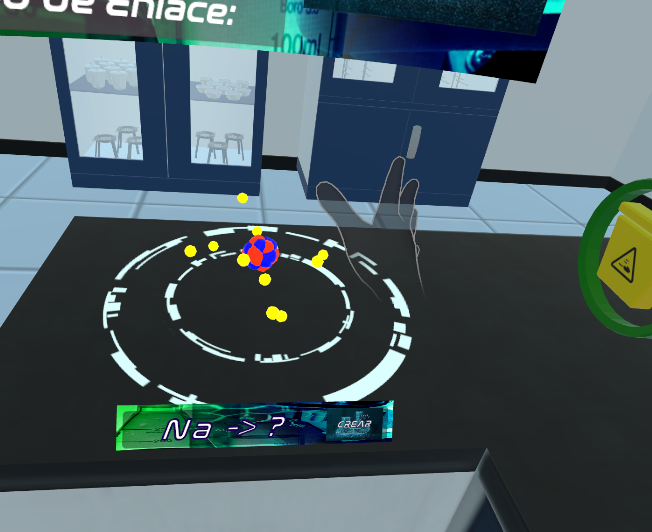
\includegraphics[width=0.5\textwidth, height = 5cm]{img/Interacciones/Zona_Creación (2).png}
        \caption{Zona de Creación}
        \label{fig:Zona de Creación}
    \end{figure}

    \item \textbf{Desechar Elementos:}  
    Lleva cualquier objeto no deseado a la zona de desecho y suéltalo (abre la mano). El sistema eliminará automáticamente el elemento.
    \begin{figure}[thbp]
        \centering
        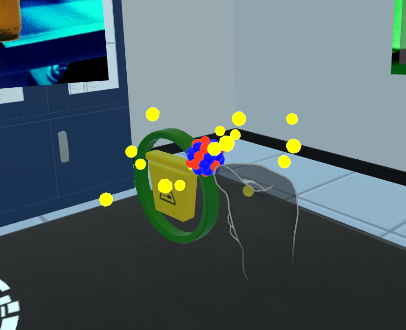
\includegraphics[width=0.5\textwidth, height = 5cm]{img/Interacciones/Eliminación.png}
        \caption{Eliminación de Elementos}
        \label{fig:Eliminación de Elementos}
    \end{figure}
    \newpage
    \item \textbf{Verter Líquidos:}  
    \begin{itemize}
        \item \textit{Vaciado:} Inclina el recipiente hasta que el líquido fluya hacia el destino deseado.  
        \item \textit{Llenado:} Derrama el líquido desde otro recipiente para llenarlo.  
    \end{itemize}
    \begin{figure}[thbp]
        \centering
        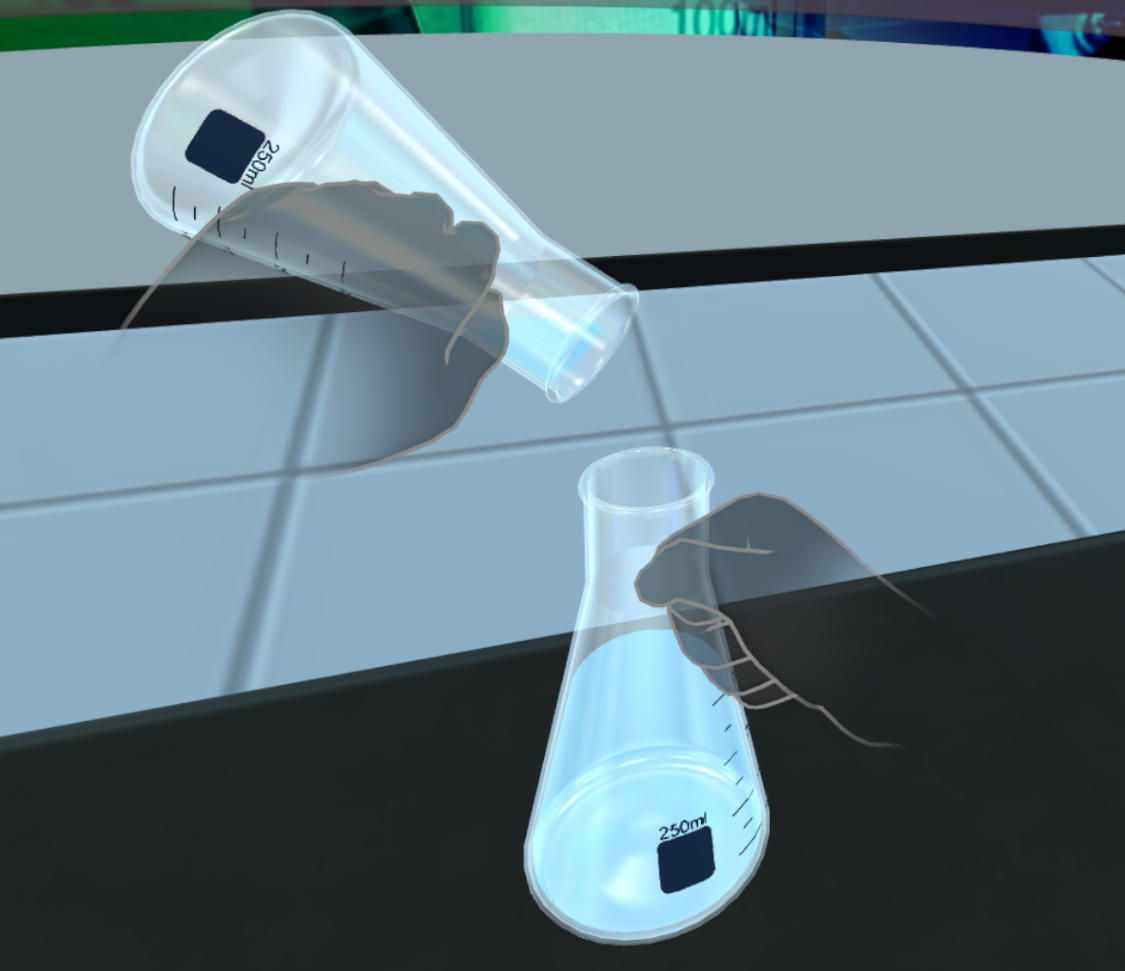
\includegraphics[width=0.5\textwidth, height = 5cm]{img/Interacciones/Vertido.png}
        \caption{Vertido y Llenado de Líquidos}
        \label{fig:Vertido y Llenado de Líquidos}
    \end{figure}
    \item \textbf{Uso del Gotero:}  
    Toma el gotero con un gesto de agarre e inclínalo sobre el recipiente para liberar las gotas.
    \begin{figure}[thbp]
        \centering
        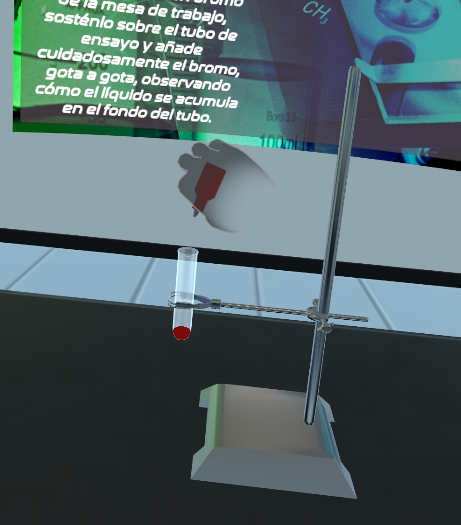
\includegraphics[width=0.5\textwidth, height = 5cm]{img/Interacciones/Agregar_Liquido.png}
        \caption{Uso de Gotero}
        \label{fig:Uso de Gotero}
    \end{figure}
    \item \textbf{Manipulación de Polvos:}  
    Usa la espátula para recoger y vaciar polvos en un recipiente:
    \begin{enumerate}
        \item Sujeta la espátula con un gesto de agarre.  
        \item Acerca la punta al contenedor de polvos para recogerlos.  
        \item Inclina la espátula sobre el recipiente objetivo para vaciarlos.  
    \end{enumerate}

    \begin{figure}[thbp]
            \centering
            \begin{subfigure}[b]{0.5\linewidth}
                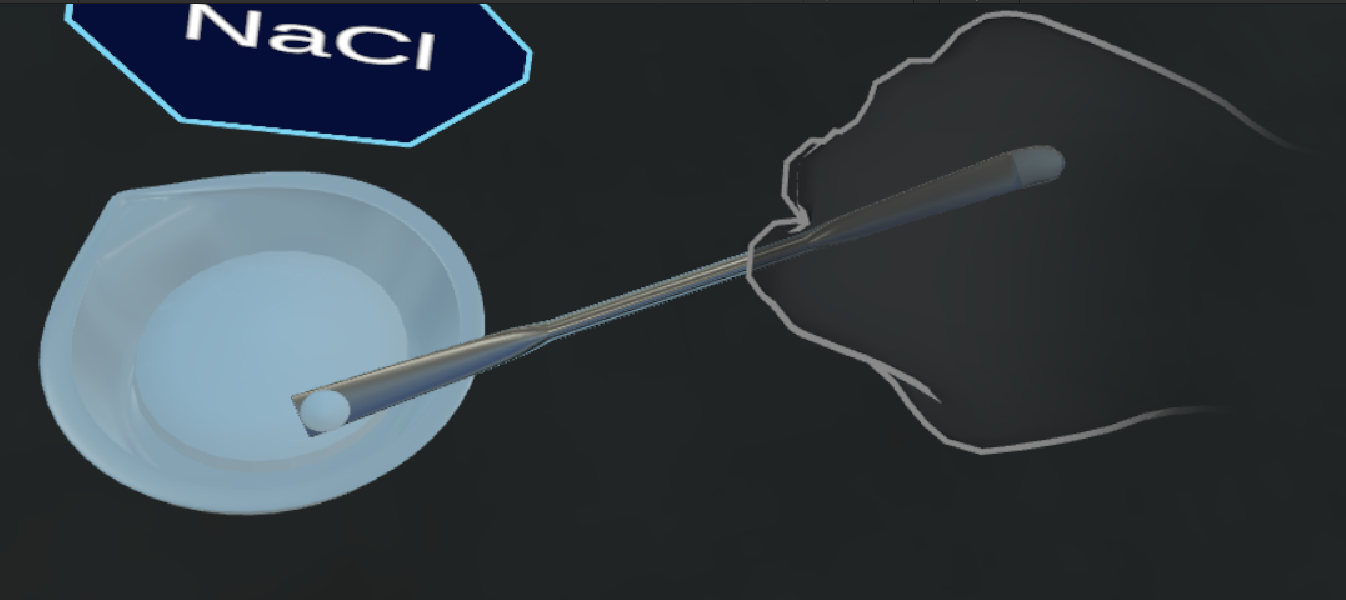
\includegraphics[width=\linewidth, height = 4cm]{img/Interacciones/Polvos1.png}
            \end{subfigure}
            \begin{subfigure}[b]{0.3\linewidth}
                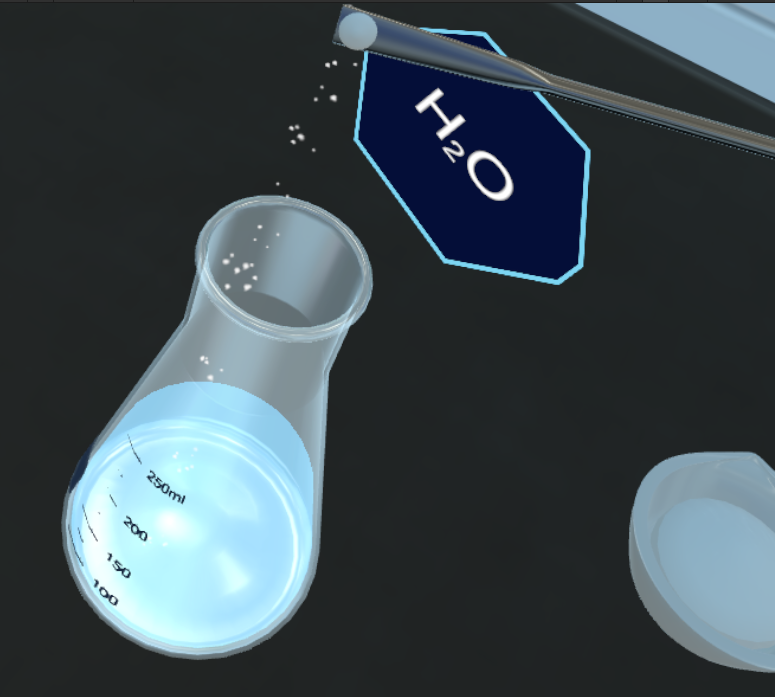
\includegraphics[width=\linewidth, height = 4cm]{img/Interacciones/Polvos2.png}
            \end{subfigure}
            \caption{Manipulación de Polvos}
        \end{figure}
    
    \item \textbf{Activar y Desactivar el Encendedor:}  
    Agita el encendedor con un movimiento rápido para encenderlo. Repite la misma acción para apagarlo.

    \item \textbf{Encender el Mechero:}  
    Una vez encendido el encendedor, acércalo a la punta del mechero. Este mostrará un efecto visual de fuego que indica que está activo.

\begin{figure}[thbp]
    \centering
    \begin{subfigure}[b]{0.4\linewidth}
        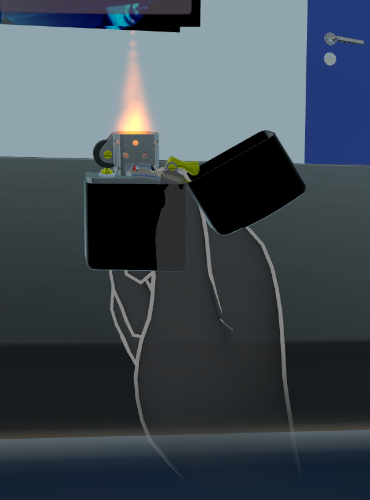
\includegraphics[width=\linewidth, height = 5cm]{img/Interacciones/Encendido01.png}
        \caption{Uso de encendedor}
        \label{fig:Encendedor}
    \end{subfigure}
    \begin{subfigure}[b]{0.4\linewidth}
        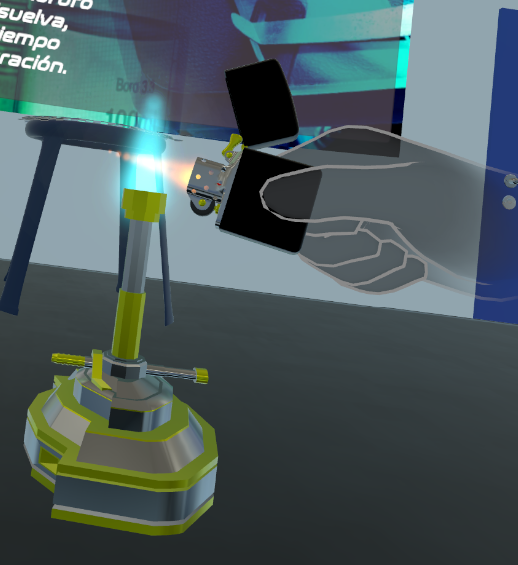
\includegraphics[width=\linewidth, height = 5cm]{img/Interacciones/Encendido02.png}
        \caption{Encendido de mechero}
        \label{fig:Mechero}
    \end{subfigure}
    \caption{Encendido diverso}
\end{figure}

    \item \textbf{Calentar Líquidos:}  
    Coloca el mechero encendido debajo del trípode con rejilla y coloca el recipiente deseado sobre la rejilla. El sistema mostrará efectos visuales como burbujeo y vapor.
    \begin{figure}[thbp]
        \centering
        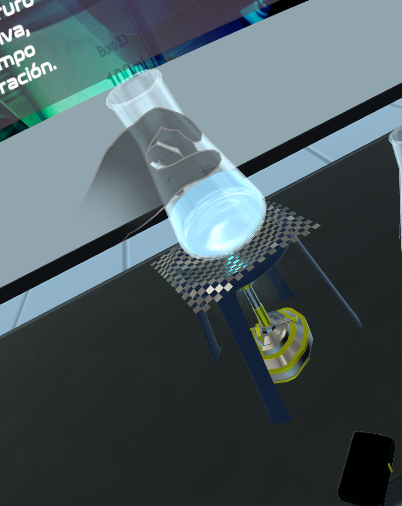
\includegraphics[width=0.5\textwidth, height = 5cm]{img/Interacciones/Calentamiento.png}
        \caption{Calentamiento de Líquidos}
        \label{fig:Calentamiento de Líquidos}
    \end{figure}
\end{itemize}
\newpage
\section{Seguridad y Advertencias}

El simulador de laboratorio de química inorgánica en realidad virtual ha sido diseñado para proporcionar una experiencia inmersiva y educativa en un entorno seguro. Sin embargo, es importante seguir estas recomendaciones para garantizar un uso adecuado y prevenir posibles inconvenientes:

\subsection{Entorno Seguro}
\begin{itemize}
    \item Asegúrate de utilizar el simulador en un espacio libre de obstáculos con un área mínima de 2x2 metros.
    \item Mantén una iluminación adecuada para que el sistema de seguimiento de manos (\textit{hand tracking}) funcione correctamente.
    \item Revisa el entorno antes de iniciar la sesión para evitar colisiones accidentales con muebles, paredes u otros objetos.
\end{itemize}

\subsection{Uso Responsable}
\begin{itemize}
    \item No utilices las gafas de realidad virtual durante períodos prolongados sin descansar. Se recomienda hacer una pausa de 10 a 15 minutos por cada 30 minutos de uso.
    \item Si experimentas mareos, náuseas, fatiga ocular o molestias físicas, interrumpe el uso de inmediato y descansa en un entorno tranquilo.
\end{itemize}

\subsection{Cuidado del Equipo}
\begin{itemize}
    \item Limpia las lentes de las gafas con un paño de microfibra suave para evitar rayaduras.
    \item Asegúrate de que las gafas estén correctamente ajustadas para evitar caídas o movimientos incómodos durante el uso.
    \item Mantén las gafas alejadas de fuentes de calor y humedad para prevenir daños en los componentes internos.
\end{itemize}

\subsection{Precauciones con el Seguimiento de Manos}
\begin{itemize}
    \item Evita realizar movimientos bruscos o rápidos que puedan causar pérdida de precisión en el seguimiento de manos.
    \item Mantén las manos visibles para el sistema en todo momento para garantizar una interacción fluida.
\end{itemize}

Estas recomendaciones están diseñadas para maximizar la seguridad y comodidad durante el uso del simulador. El incumplimiento de estas indicaciones puede afectar negativamente la experiencia y, en algunos casos, causar daños al usuario o al equipo.
